\documentclass{article}
\usepackage{amsmath}
\usepackage{amsfonts}
\usepackage{amssymb}

\usepackage{enumitem}

\usepackage{graphicx}

\usepackage{minted}

\usepackage{hyperref}

\begin{document}

\tableofcontents

\newpage
\setcounter{section}{1}
\section{Preliminaries}
\subsection{Data Manipulation}
\begin{enumerate}
\item Run the code in this section. Change the conditional statement \texttt{X == Y} to \texttt{X < Y} or \texttt{X > Y}, and then see what kind of tensor you can get.
\item Replace the two tensors that operate by element in the broadcasting mechanism with other shapes, e.g., 3-dimensional tensors. Is the result the same as expected?
\end{enumerate}

\subsection{Data Preprocessing}
\begin{enumerate}
    \item Try loading datasets, e.g., Abalone from the UCI Machine Learning Repository and inspect their properties. What fraction of them has missing values? What fraction of the variables is numerical, categorical, or text?

    \item Try out indexing and selecting data columns by name rather than by column number. The pandas documentation on indexing has further details on how to do this.

    \item How large a dataset do you think you could load this way? What might be the limitations? Hint: consider the time to read the data, representation, processing, and memory footprint. Try this out on your laptop. What changes if you try it out on a server?

    \item How would you deal with data that has a very large number of categories? What if the category labels are all unique? Should you include the latter?

    \item What alternatives to pandas can you think of? How about loading NumPy tensors from a file? Check out Pillow, the Python Imaging Library.
\end{enumerate}



\subsection{Linear Algebra}
\begin{enumerate}
    \item Prove that the transpose of the transpose of a matrix is the matrix itself: \\
    $$(A^T)^T = A$$
    	\begin{itemize}
    		\item The transpose per definition satisfies $(A^T)_{ij} = A_{ji}$ for all $i, j$. As such $((A^T)^T)_{ij} = (A^T)_{ji} = A_{ij}$, which shows that $(A^T)^T = A$.
    	\end{itemize}

    \item Given two matrices $A$ and $B$, show that sum and transposition commute: \\
    $$(A + B)^T = A^T + B^T$$
    	\begin{itemize}
    		\item Let $i, j$ be arbitrary valid indiced then
    		$$((A + B)^T)_{ij} = (A + B)_{ji} = A_{ji} + B_{ji} = (A^T)_{ij} + (B^T)_{ij}$$
    		holds, this proves that $(A + B)^T = A^T + B^T$.
    	\end{itemize}

    \item Given any square matrix $A$, is $A + A^T$ always symmetric? Can you prove the result by using only the result of the previous two exercises?
    	\begin{itemize}
    		\item A square matrix $B$ is symmetric if and only if $B^T = B^T$. In view of the previous two exercises the symmetry of $A + A^T$ immediately follows:
    		$$
    		(A + A^T)^T \overset{2}{=} A^T + (A^T)^T \overset{1}{=} A^T + A = A + A^T.
    		$$ 
    		where in the last step we have used that matrix addition is commutative.
    	\end{itemize}

    \item We defined the tensor $X$ of shape $(2, 3, 4)$ in this section. What is the output of \texttt{len}(X)? Write your answer without implementing any code, then check your answer using code.
    	\begin{itemize}
    		\item I assume that internally the tensor $X$ is represented as $((\mathbb{R}^4)^3)^2$, which would then give the length as $2$.
    	\end{itemize}

    \item For a tensor \texttt{X} of arbitrary shape, does \texttt{len}(X) always correspond to the length of a certain axis of \texttt{X}? What is that axis?

    \item Run \texttt{A / A.\texttt{sum}(axis=1)} and see what happens. Can you analyze the reason?

    \item When traveling between two points in downtown Manhattan, what is the distance that you need to cover in terms of the coordinates, i.e., in terms of avenues and streets? Can you travel diagonally?
    	\begin{itemize}
    		\item This problem wants me to state the manhattan distance:
    		$$
    		d((x_1, \dots, x_n), (y_1, \dots, y_n)) = \sum_{i = 1}^n |x_i - y_i|.
    		$$
    	\end{itemize}

    \item Consider a tensor with shape $(2, 3, 4)$. What are the shapes of the summation outputs along axis $0$, $1$, and $2$?

    \item Feed a tensor with $3$ or more axes to the $\texttt{linalg.norm}$ function and observe its output. What does this function compute for tensors of arbitrary shape?

    \item Define three large matrices, say $A$, $B$, and $C$, for instance initialized with Gaussian random variables. You want to compute the product $ABC$. Is there any difference in memory footprint and speed, depending on whether you compute $AB$ or $BC$ first? Why?
    \begin{itemize}
    	\item Let $A \in \mathbb{R}^{r \times s}, B \in \mathbb{R}^{s \times t}$ and $C \in \mathbb{R}^{t \times u}$. We are assuming the naive matrix multiplication algorithm is used, then to calculate $A \cdot B \in \mathbb{R}^{r \times t}$ we need $O(rst)$ steps and similiarly for $B \cdot C \in \mathbb{R}^{s \times u}$ we need $O(s t u)$ steps. To then calculate $(A \cdot B) \cdot C$ we need $O(rtu)$ steps and to calculate $A \cdot (B \cdot C)$ we need $O(rsu)$. As such in total we need $O(rst + rtu) = O(rt(u + s))$ to calculate $(A \cdot B) \cdot C$ and $O(stu + rsu) = O(su(t + r))$.
    \end{itemize}

    \item Define three large matrices, say $A$, $B$, and $C$. Is there any difference in speed depending on whether you compute $AB$ or $BA$ first? Why? What changes if you initialize $B$ without cloning memory? Why?

    \item Define three matrices, say $A$, $B$, and $C$. Constitute a tensor with $3$ axes by stacking $A$, $B$, and $C$. What is the dimensionality? Slice out the second coordinate of the third axis to recover $B$. Check that your answer is correct.
\end{enumerate}


\subsection{Calculus}
\begin{enumerate} 
\item So far we took the rules for derivatives for granted. Using the definition and limits prove the properties for (i) $f(x) = c$, (ii) $x^n$, (iii) $e^x$ and (iv) $\log x$.
	\begin{itemize}
	\item We note that $f_1(x) = c$ satisfies $f_1(x) - f_1(x_0) = 0$ for all $x, x_0 \in \mathbb{R}$, which allows us to calculate:
	$$
	\lim_{x \rightarrow x_0} \frac{f(x) - f(x_0)}{x - x_0} = \lim_{x \rightarrow x_0} \frac{c - c}{x - x_0} = 0.
	$$
	\item Note that $f_2(x) = x^n$ is a polynomial and $F(x, y) = x^n - y^n$ is a polynomial in two variables which satisfies $F(x, x) = 0$ as such we can factor out $x - y$ from $F(x, y)$, it can inductively be shown that $F(x, y) = (x - y) \sum_{i = 0}^{n - 1} x^i y^{n - 1 - i}$. With this we can now calculate
	\begin{align*}
	\lim_{x \rightarrow x_0} \frac{f(x) - f(x_0)}{x - x_0} &= \lim_{x \rightarrow x_0} \frac{x^n - x_0^n}{x - x_0} \\
	&= \lim_{x \rightarrow x_0} \frac{(x - x_0)\left(\sum_{i = 0}^{n - 1} x^i x_0^{n - 1 - i}\right)}{x - x_0} \\
	&= \lim_{x \rightarrow x_0} \sum_{i = 0}^{n - 1} x^i x_0^{n - 1 - i} \\
	&= \sum_{i = 0}^{n - 1} x_0^{n - 1} = \left(\sum_{i = 0}^{n - 1} 1\right) x_0^{n - 1} = n x_0^{n - 1}.
	\end{align*}
	\item This problem depends on which representation of the exponential is used. In the book they defined it via its differential equation, i.e. $f_3(x) = e^x$ is the unique solution of $y' = y$ with initial value $y(0) = 1$, but then there is nothing to show here. Instead we'll use the power series representation
	$$
	\sum_{n = 0}^\infty \frac{x^n}{n!}
	$$
	of $f_3(x)$. It is easily verifiable that this power series is absolutely convergent, which allows us to show that
	\begin{align*}
	f_3(x) - f_3(x_0) &= \sum_{n = 0}^\infty \frac{x^n}{n!} - \sum_{n = 0}^\infty \frac{x_0^n}{n!} \\
	&= \sum_{n = 0}^\infty \frac{x^n - x_0^n}{n!} = (x - x_0) + \sum_{n = 2}^\infty\frac{x^n - x_0^n}{n!}
	\end{align*}
	holds. We can use the calculation for $f_2(x)$ so write this as
	\begin{align*}
	f_3(x) - f_3(x_0) &= (x - x_0) + (x - x_0) \sum_{n = 2}^\infty \frac{\sum_{j = 0}^{n - 1} x^j x_0^{n - 1 - j}}{n!} \\
	&= (x - x_0) \left(1 + \frac{x + x_0}{2} + \dots \right)
	\end{align*}
	In total this proves that
	$$
	f_3'(x_0) = \lim_{x \rightarrow x_0} \left(1 + \frac{x + x_0}{2} + \dots \right) = \sum_{j = 0}^\infty \frac{x_0^j}{j!} = f_3(x_0)
	$$
	\item Consider $f_4(x) = \log(x)$ and note that $f_3 \circ f_4 = \operatorname{id}$. Using the chain rule then yields
	$$
	1 = f_3' \circ f_4 \cdot f_4'
	$$
	and because $f_3' = f_3$ this reduces to
	$$
	f_4' = \frac{1}{f_3 \circ f_4}
	$$
	so that
	$$
	f_4'(x) = \frac{1}{x}.
	$$
	\end{itemize}

\item In the same vein, prove the product, sum, and quotient rule from first principles.
	\begin{itemize}
	\item Using a similiar construction to the triangle inequality we can write
	\begin{align*}
	(fg)(x) - (fg)(y) &= f(x)g(x) - f(y)g(y) \\
	&= f(x)g(x) - f(x)g(y) + f(x)g(y) - f(y)g(y) \\
	&= f(x)(g(x) - g(y)) + (f(x) - f(y))g(y),
	\end{align*}
	from which we can conclude
	\begin{align*}
	\lim_{x \rightarrow y} \frac{fg(x) - fg(y)}{x - y} &= \lim_{x \rightarrow y} \frac{f(x)(g(x) - g(y)) + (f(x) - f(y))g(y)}{x - y} \\
	&= \lim_{x \rightarrow y} f(x) \frac{g(x) - g(y)}{x - y} + \frac{f(x) - f(y)}{x - y} g(y) \\
	&= f(y) g'(y) + f'(y)g(y).
	\end{align*}
	This can also be expressed as
	$$
	(fg)' = f'g + fg',
	$$
	which is what was to be shown.
	\item The sum formula immediately follows from the linearity of $\lim$.
	\item The quotient formula immediately follows from the product rule by noting that $\frac{f}{g} = f \cdot \frac{1}{g}$ as well as $\left(\frac{1}{g(x)}\right)' = -\frac{g'(x)}{g^2(x)}$. To see this apply the product rule on $1 = g(x) \frac{1}{g(x)}$.
	\end{itemize}

\item Prove that the constant multiple rule follows as a special case of the product rule.
	\begin{itemize}
	\item $(cf(x))' = c' f(x) + c f'(x)$, we have already shown that $c' = 0$ so that $(cf)' = cf'$.
	\end{itemize}

\item Calculate the derivative of $f(x) = x^x$. 
	\begin{itemize}
	\item We assume that $x > 0$ then $f(x) = x^x = e^{x \log(x))}$. Let $u(x) = x \log(x)$ then $u'(x) = \log(x) + x \cdot \frac{1}{x} = \log(x) + 1$. This allows us to write $f(x) = e^{u(x)}$, the derivative of $f$ is then, by using the chain rule and the fact that $\frac{d}{dx} e^x = e^x$, given by
	$$
	f'(x) = u'(x) e^{u(x)} = (1 + \log(x))e^{x \log(x)} = (1 + \log(x))x^x.
	$$
	\end{itemize}

\item What does it mean that $f'(x) = 0$ for some $x$? Give an example of a function $f$ and a location $x$ for which this might hold.
	\begin{itemize}
	\item Depending on the neighboring values (or if it's $C^2$ on the sign of the second derivative), that $x$ is either a minimizer ($x = 0$ for $f(x) = x^2$), a maximizer ($x = 0$ for $f(x) = -x^2$) or a saddle point ($x = 0$ for $f(x) = x^3$).
	\end{itemize}

\item Plot the function $y = f(x) = x^3 - \frac{1}{x}$ and plot its tangent line at $x = 1$.
	\begin{itemize}
	\item The derivative of $f$ is given by $f'(x) = 3x^2 + \frac{1}{x^2}$, evaluated at $x = 1$ this yields a slope of $f'(1) = 3 + 1 = 4$, so the tangent line is given by $y(x) = 4x + b$ where $b$ is such thatt $y(1) = 4 + b = f(1) = 0$ so that $b = -4$. In total this means the tangent line at $x = 1$ is given by
	$$
	y(x) = 4x - 4.
	$$
	\begin{center}
    	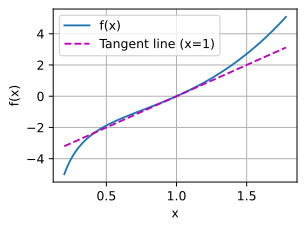
\includegraphics[width=0.6\textwidth]{Images/2_4_6.png}
    \end{center}
	\end{itemize}

\item Find the gradient of the function $f(x) = ||x||_2$? What happens for $x = 0$?
	\begin{itemize}
	\item Note that if $x = (x_1, \dots, x_n)$ then $g(x) := f(x)^2 = ||x||_2^2 = \sum_{i = 1}^n x_i^2$. It follows that for $x \neq 0$ the corresponding partial derivates are simply given by
	$$
	\frac{\partial}{\partial x_j} f(x)^2 = \frac{\partial}{\partial x_j} \sum_{i = 1}^n x_i^2 = 2 x_i.
	$$
	This shows that $\nabla g(x) = 2 x$. Furthermore $\frac{\partial}{\partial x_j} g(x) = \frac{\partial}{\partial x_j} f(x)^2 = 2 \frac{\partial f}{\partial x_j} \cdot f(x)$. With that we can calculate
	$$
	2x = 2 f(x) \nabla f \iff \nabla f = \frac{x}{f(x)} = x / ||x||.
	$$
	Note that this construction breaks down at $x = 0$ as we would divide by $0$. But this is not surprising because $x \mapsto \sqrt{x}$ is not differentiable at $0$ and $f(x) = \sqrt{g(x)}$.
	\end{itemize}

\item Can you write out the chain rule for the case where $u = f(x, y, z)$ and $x = x(a, b), y = y(a, b)$ and $z = z(a, b)$?
	\begin{itemize}
	\item We can write $u(a, b) = f(x(a, b), y(a, b), z(a, b))$ and with that
	$$
	\frac{\partial}{\partial a} u(a, b) = \frac{\partial f}{\partial x}(\dots) \cdot \frac{\partial x}{\partial a} + \frac{\partial f}{\partial y}(\dots) \cdot \frac{\partial y}{\partial a} + \frac{\partial f}{\partial z}(\dots) \cdot \frac{\partial z}{\partial a},
	$$
	which can be expressed as
	$$
	(\nabla f)(x(a, b), y(a, b), z(a, b)) \cdot \nabla_a (x, y, z).
	$$
	Similiarly once can show taht
	$$
	(\nabla f)(x(a, b), y(a, b), z(a, b)) \cdot \nabla_b (x, y, z).
	$$
	With that it follows that
	$$
	\nabla u(a, b) = (\nabla f, \nabla f)^t \cdot (D(x, y, z)).
	$$
	\end{itemize}

\item Given a function $f(x)$ that is invertible, compute the derivative of its inverse $f^{-1}(x)$. Here we have that $f^{-1}(f(x)) = x$ and conversely $f(f^{-1}(y)) = y$. Hint: Use these properties in your derivation.
	\begin{itemize}
		\item We can calculate
		$$
		1 = \frac{\partial}{\partial x} x = \frac{\partial}{\partial x} f^{-1}(f(x)) = (f^{-1})'(f(x)) f'(x),
		$$
		which can be rewritten as
		$$
		(f^{-1})'(f(x)) = \frac{1}{f'(x)}.
		$$
		If we write $y = f(x)$ this becomes
		$$
		(f^{-1})'(y) = \frac{1}{f'(x)}.
		$$
	\end{itemize}
\end{enumerate}

\begin{minted}{python}
# Code for Ex 6
def f(x):
    return x ** 3 - 1 / x

x = np.arange(0.2, 1.8, 0.02)
y = [x ** 3 - 1 / x, 4 * x - 4]
plot(x, y, 'x', 'f(x)', legend=['f(x)', 'Tangent line (x=1)'])
\end{minted}

\subsection{Automatic Differentiation}
\begin{enumerate}
\item Why is the second derivative much more expensive to compute than the first derivative?
	\begin{itemize}
		\item The derivative can be approximated by sampling two points, the second derivative needs more points. If we consider the second derivative as the derivative of the derivative then we need to sample two points at each of the original sampling points, which more than doubles the workload. Note that the second derivative is the average rate of change of the rate of change of the two sample points, symbolically:
		$$
		f'(x_0) \sim f(x_0 + \varepsilon) - f(x_0 - \varepsilon)
		$$
		and
		\begin{align*}
		f'(x_0 + \varepsilon) = f(x_0 + 2\varepsilon) - f(x_0),&&f'(x_0 - \varepsilon) = f(x_0) - f(x_0 - 2\varepsilon).
		\end{align*}
		From this it can be seen that the second derivative can be expressed as
		\begin{align*}
		f''(x_0) &= f'(x_0 + \varepsilon) - f'(x_0 - \varepsilon) \\
		&= f(x_0 + 2\varepsilon) - f(x_0) - (f(x_0) - f(x_0 - 2\varepsilon)) \\
		&= f(x_0 + 2\varepsilon) - 2f(x_0) + f(x_0 - 2\varepsilon)).
		\end{align*}
		There are much better choice for sampling points to get faster numerical convergence, but this is beyond the scope of what we're doing here. 
	\end{itemize}
\item After running the function for backpropagation, immediately run it again and see what happens. Why?
	\begin{itemize}
		\item An error is thrown, because the gradient tape gets wiped.
	\end{itemize}
\item In the control flow example where we calculate the derivative of d with respect to a, what would happen if we changed the variable a to a random vector or a matrix? At this point, the result of the calculation f(a) is no longer a scalar. What happens to the result? How do we analyze this?
	\begin{itemize}
		\item My guess would be that we just get a higher order tensor as our gradient. Yeah, we get a higher order tensor, equal to the dimension of $a$. For the function in question all its entries are the same.
	\end{itemize}
\item Let $f(x) = \sin(x)$. Plot the graph of $f$ and its derivative $f'$. Do not exploit the fact that $f'(x) = \cos(x)$ but rather use automatic differentiation to get the result.
	\begin{itemize}
		\item The code can be found below, the plot is as follows:
		\begin{center}
		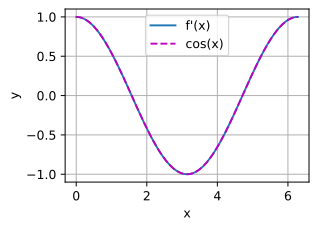
\includegraphics[width=0.6\textwidth]{Images/2_5_4.png}
		\end{center}
	\end{itemize}
\item Let $f(x) = ((\log x^2) \cdot \sin x) + x^{-1}$. Write out a dependency graph tracing results from $x$ to $f(x)$.
	\begin{itemize}
		\item I'm not entirely sure what they are looking for, but maybe it's like the type of graph you'd draw for a parser which tries to understand mathematical operations. This notation I just made up, it's useable but I doubt it's standard.
		$$
		\begin{aligned}
		f(x) &\rightarrow \{(\log x^2) \cdot \sin x, x^{-1}, +\} \\
		&\rightarrow \{\{\log x^2, \sin x, \cdot\}, x^{-1}, +\} \\
		&\rightarrow \{\{x^2, \log, \circ\}, \sin x, \cdot\}, x^{-1}, +\}
		\end{aligned}
		$$
	\end{itemize}
\item Use the chain rule to compute the derivative $f'$ of the aforementioned function, placing each term on the dependency graph that you constructed previously.
	\begin{itemize}
		\item
		$$
		\begin{aligned}
		df &= d\{\{x^2, \log, \circ\}, \sin x, \cdot\}, x^{-1}, +\} \\
		&= \{d\{x^2, \log, \circ\}, \sin x, \cdot\}, d(x^{-1}),+\} \\
		&= \{d\{x^2, \log, \circ\} \cdot \sin(x) + \{x^2, \log, \circ\} \cdot d\sin(x), \sin x, \cdot\}, -x^{-2},+\} \\
		&= \{d\{x^2, \log, \circ\} \cdot \sin(x) + \{x^2, \log, \circ\} \cdot d\sin(x), \sin x, \cdot\}, -x^{-2},+\} \\
		&= \{\frac{2x}{x^2} \cdot \sin(x) + \{x^2, \log, \circ\} \cdot \cos(x), \sin x, \cdot\}, -x^{-2},+\} \\
		&= \dots
		\end{aligned}
		$$
		Something like this, you get the idea.
	\end{itemize}
\item Given the graph and the intermediate derivative results, you have a number of options when computing the gradient. Evaluate the result once starting from $x$ to $f$ and once from $f$ tracing back to $x$. The path from $x$ to $f$ is commonly known as \textit{forward differentiation}, whereas the path from $f$ to $x$ is known as \textit{backward differentiation}.
\item When might you want to use forward differentiation and when backward differentiation? Hint: consider the amount of intermediate data needed, the ability to parallelize steps, and the size of matrices and vectors involved.
\end{enumerate}

\begin{minted}{python}
# Code for Ex 4
num_steps = 100
my_tau = 2 * tf.constant(3.14159265358979323846, dtype = tf.float32)
x = tf.linspace(0.0, my_tau, num_steps)
x_var = tf.Variable(x)
with tf.GradientTape() as t:
    y = tf.math.sin(x_var)
x_grad = t.gradient(y, x_var)
assert(tf.reduce_all(tf.abs(x_grad - tf.math.cos(x)) < 0.001))

y = [x_grad, tf.math.cos(x)]
printing.plot(x, y, "x", "y", legend=["f'(x)", "cos(x)"])
\end{minted}

\subsection{Probability and Statistics}
This might be a bit too technical for the course, but to remind myself of the background. Let $(\Omega, \mathcal{A}, P)$ be a probability space, this is a measure space (i.e. $\Omega$ is some set, $\mathcal{A}$ is a sigma algebra on $\Omega$ and $P$ is a measure, i.e. a $\sigma$-additive function $P : \mathcal{A} \rightarrow [0, +\infty)$ which satisfies $P(\emptyset) = 0$), where the measure is a probability function, i.e. $P(\Omega) = 1$. Recall that this means that probability theory is only interested in the theory of finite measures.

A random variable is a measureable function $X : \Omega \rightarrow \mathbb{R}$. We call the elements of the sigma algebra an event (and the sigma-algebra itself the event space) and the elements of $\Omega$ a sample (and $\Omega$ itself a sample space). The expression
$$
P\left(\lim_{n \rightarrow \infty} X_n = \alpha\right) = p
$$
is simply shorthand for
$$
P\left(\{\omega \in \Omega : \lim_{n \rightarrow \infty} X_n(\omega) = \alpha\}\right) = p.
$$
\begin{enumerate}
	\item Give an example where observing more data can reduce the amount of uncertainty about the outcome to an arbitrarily low level.
	\begin{itemize}
		\item Consider flipping a weighted coin, whose probability to land on heads is given by $p_H \in (0, 1)$. Let $(X_i)_{i \in \mathbb{N}}$ be a sequence of random variables where $X_i \in \{0, 1\}$ and is $1$ if the $i$th flip landed on heads. Counting the outcome of the first $n$ flips yields the random variable
		$$
		\tilde{X}_n := \sum_{i}^n X_i.
		$$
		Note that
		$$
		P\left(\lim_{n \rightarrow \infty} \frac{\tilde{X}_n}{n} \neq p_H\right) = 0,
		$$
		or if we consider the running average $Y_n := \frac{1}{n} \tilde{X}_n$ this can be expressed as
		$$
		P\left(\lim_{n \rightarrow \infty} Y_n = p_H\right) = 1.
		$$
	\end{itemize}

	\item Give an example where observing more data will only reduce the amount of uncertainty up to a point and then no further. Explain why this is the case and where you expect this point to occur.
	\begin{itemize}
		\item Sticking to the same example as before, flipping a fair coin. If the question is what is the probability that the coin is fair, we get a convergence to $100\%$. But if we instead ask what is the probability that the next flip will be heads we can only have a certainty of $50\%$ that it will be heads. If $p$ denotes the probability of heads, we can establish this value arbitrarily close, but the probability of getting heads will still be $p$. This uncertainty is inherent to the system. Using the notation of the book, this is an example of aleatoric uncertainty, while the actual value of $p$ is epistemic uncertainty.
	\end{itemize}
	\item We empirically demonstrated convergence to the mean for the toss of a coin. Calculate the variance of the estimate of the probability that we see a head after drawing $n$ samples.
		\begin{itemize}
			\item Let $X_i \in \{0, 1\}$ denote if the $i$th flip landed on head and consider 
			$$
			\tilde{X}_n := \sum_{i = 1}^n X_i.
			$$
			We are interested in $P(\tilde{X}_n \geq 1)$. Note that for $k \in {0, \dots, n}$ the statement $\tilde{X}_n = k$ is equivalent to there being exactly $k$ heads, which means we have $k$ heads and $n - k$ tails. Denote by $p$ the probability of getting heads, then flipping $k$ heads and $n - k$ tails has a probability of
			$$
			p^k (1 - p)^{n - k}
			$$
			and because the order of those doesn't matter we have to multiply this with the number of permutations, i.e., we are interested in how many arrangements there are to distribute $k$ (or equivalently $n - k$) elements in $n$ slots. This is exactly the binomial coefficient
			$$
			\binom{n}{k} = \frac{n!}{k! (n - k)!}.
			$$
			In total this means
			$$
			P(\tilde{X}_n = k) = \binom{n}{k} p^k (1 - p)^{n - k}.
			$$

			Looking back on it now, I just realized that the $X_i$ are all independent as such
			$$
			E[\tilde{X}_n] = E\left[\sum_{i = 1}^n X_i\right] = \sum_{i = 1}^n E[X_i] = \sum_{i = 1}^n p = np.
			$$

			Alternatively the expected value of $\tilde{X}_n$ can then be calculated directly as
			$$
			\begin{aligned}
			E[\tilde{X}_n] &= \sum_{k = 0}^n kP(\tilde{X}_n = k) \\
			&= \sum_{k = 0}^n k \binom{n}{k} p^k (1 - p)^{n - k} \\
			&= \sum_{k = 0}^n k \binom{n}{k} p^k (1 - p)^{n - k}.
			\end{aligned}
			$$
			This can be explicitly calculated to be $np$, we're only going to prove the case where $p = 1 - p = 0.5$, in that case
			$$
			\begin{aligned}
			E[\tilde{X}_n] &= \sum_{k = 0}^n k \binom{n}{k} 2^{-n}
			&= 2^{-n} \sum_{k = 0}^n k \binom{n}{k} \\
			&\overset{*}{=} 2^{-n} 2^{n - 1} = n / 2 = pn.
			\end{aligned}
			$$
			What remains to be shown is that $(*)$ holds. This can be done inductively, it obviously holds for $n = 1$. Now suppose the identity holds for some $n \in \mathbb{N}$, then
			$$
			\sum_{k = 0}^{n + 1} k \binom{n + 1}{k} = (n + 1) + \sum_{k = 0}^n k \binom{n + 1}{k},
			$$
			using Pascal's triangle equality we can write
			$$
			\binom{n + 1}{k} = \binom{n}{k} + \binom{n}{k - 1}.
			$$
			With this we can then calculate
			$$
			\begin{aligned}
			\sum_{k = 0}^{n + 1} k \binom{n + 1}{k} &= (n + 1) + \sum_{k = 0}^n k \binom{n + 1}{k} \\
			&= (n + 1) + \sum_{k = 0}^n k \left[ \binom{n}{k} + \binom{n}{k - 1} \right] \\
			&= (n + 1) + \sum_{k = 0}^n k \binom{n}{k} + \sum_{k = 0}^n k \binom{n}{k - 1} \\
			&= (n + 1) + \sum_{k = 0}^n k \binom{n}{k} + \sum_{k = 0}^{n - 1} (k + 1) \binom{n}{k} \\
			&= (n + 1) + \sum_{k = 0}^n k \binom{n}{k} + \sum_{k = 0}^{n - 1} k \binom{n}{k} + \sum_{k = 0}^{n - 1} \binom{n}{k} \\
			&= (n + 1) + \sum_{k = 0}^n k \binom{n}{k} + \sum_{k = 0}^n k \binom{n}{k} + \sum_{k = 0}^{n - 1} \binom{n}{k} - n \\
			&= 2 \sum_{k = 0}^n k \binom{n}{k} - n + \sum_{k = 0}^n \binom{n}{k} - 1.
			\end{aligned}
			$$
			Applying the well-known identity
			$$
			\sum_{k = 0}^n \binom{n}{k} = 2^n
			$$
			and the induction hypothesis to this yields
			$$
			2 (2^{n - 1}) + 2^n = 2^{n + 1}.
			$$
			By induction it then follows that for all $n \in \mathbb{N}$ the identity
			$$
			\sum_{k = 0}^n k \binom{n}{k} = 2^n
			$$
			holds.
			\item Just as for the expected value
			$$
			\operatorname{Var}[\tilde{X}_n] = \sum_{i = 1}^n \operatorname{Var}[X_i] = np(1 - p).
			$$
		\end{itemize}
		\begin{enumerate}
			\item How does the variance scale with the number of observations?
				\begin{itemize}
					\item It scales linearly.
				\end{itemize}
			\item Use Chebyshev's inequality to bound the deviation from the expectation.
				\begin{itemize}
					\item For $p = 1/2$ the mean is $\mu = n / 2$ and the standard deviation is $\sigma = \sqrt{n} / 2$. Applying Chebychev's inequality with these values and $k > 0$ yields
					$$
					P\left(\left|\tilde{X}_n - \frac{n}{2}\right| \geq k \frac{\sqrt{n}}{2}\right) \leq \frac{1}{k^2}.
					$$
					For example for $n = 16$ and $k = 2$ this becomes
					$$
					P(|\tilde{X}_{16} - 8| \geq 4) \leq \frac{1}{4},
					$$
					inverting this statement then proves that $P(6 \leq \tilde{X}_{16} \leq 10) \geq \frac{3}{4}$, i.e., there is a more than $75\%$ chance that on flipping $16$ (fair) coins we have at least $6$ and at most $10$ heads.
				\end{itemize}
			\item How does it relate to the central limit theorem?
				\begin{itemize}
					\item $$\lim_{n \rightarrow \infty} \frac{\tilde{X}_n - n / 2}{\sqrt{n} / 2}$$ converges to the standard normal distribution.
				\end{itemize}
		\end{enumerate}
	\item Assume that we draw samples from a probability distribution with zero mean and unit variance. Compute the averages
	$$
	z_m = m^{-1} \sum_{i = 1}^m X_i.
	$$
	Can we apply Chebychev's inequality for every $z_m$ independently? Why not?
		\begin{itemize}
			\item I'll assume we're talking about $X_i$ with finite amounts of values. The $X_i$ are independent so
			$$
			E[z_m] = E[m^{-1}\sum_i^m X_i] = m^{-1} \sum_{i = 1}^m \underbrace{E[X_i]}_{=\ 0} = 0.
			$$
			No, we can't apply Chebychev's inequality independently because $z_{m + 1} = z_m + X_{m + 1}$ as such $z_m$ and $z_{m + 1}$ are not independent.
		\end{itemize}
	\item Given two events with probability $P(\mathcal{A})$ and $P(\mathcal{B})$ compute upper and lower bounds on $P(\mathcal{A} \cup \mathcal{B})$ and $P(\mathcal{A} \cap \mathcal{B})$. Hint: graph the situation using a Venn diagram.
		\begin{itemize}
			\item Using a Venn diagram we can immediately see that
			$$
			\max\{P(A), P(B) \} \leq P(A \cup B) = P(A) + P(B) - P(A \cap B) \leq P(A) + P(B),
			$$
			and
			$$
			P(A) + P(B) - 1 \leq P(A \cap B) \leq \min\{P(A), P(B)\}
			$$
			holds.
		\end{itemize}
	\item Assume that we have a sequence of random variables, say $A, B$, and $C$, where $B$ only depends on $A$, and $C$ only depends on $B$, can you simplify the joint probability $P(A, B, C)$? Hint: this is a Markov chain.
		\begin{itemize}
			\item Note that $P(A, B)$ is just shorthand for $P(A \cap B)$.
			\begin{align*}
			P(A, B, C) &= P(A|B, C) P(B, C) \\
			&= P(A|B) P(B, C) \\
			&= P(A|B) P(B|C) P(C)
			\end{align*}
			where we have used (2.6.1) from the book, as well as because $A$ and $C$ are independent it follows that $P(A|B, C) = P(A|B)$. This can be expressed more generally, if we have a collection of random variables $X_i$ such that
			$$
			P(X_{i + 1} | X_i, X_{i - 1}, \dots, X_1) = P(X_{i + 1}| X_i),
			$$
			i.e. $X_{i + 1}$ only "remembers" the previous variable then
			$$
			P(X_n, \dots, X_1) = P(X_n|X_{n - 1})P(X_{n - 2}|X_{n - 3})\cdot \dots \cdot P(X_1|X_0)P(X_0).
			$$
		\end{itemize}
	\item In Section 2.6.5, assume that the outcomes of the two tests are not independent. In particular assume that either test on its own has a false positive rate of $10\%$ and a false negative rate of $1\%$. That is, for $i = 1, 2$ assume that $P(D_i = 1 | H = 0) = 0.1$ and that $P(D_i = 0 | H = 1) = 0.01$. Moreover, assume that for $H = 1$ (infected) the test outcomes are conditionally dependent, i.e., that 
	$$
	P(D_1, D_2|H = 1) = P(D_1 | H = 1)P(D_2 | H = 1)
	$$
	but for healthy patients the outcomes are coupled via $P(D_1 = 1, D_2 = 1| H = 0) = 0.02$.
	\begin{enumerate}
		\item Work out the joint probability table for $D_1$ and $D_2$ given $H = 0$ based on the information you have so far.
			\begin{itemize}
				\item
					\begin{center}
						\begin{tabular}{|c|c|c|} \hline
						Joint Probability ($H = 0$) & $D_2 = 1$ & $D_2 = 0$ \\ \hline
						$D_1 = 1$ & 0.02 & b \\ \hline
						$D_1 = 0$ & a & b \\ \hline
						\end{tabular}
					\end{center}
			\end{itemize}
		\item Derive the probability of the patient being positive $(H = 1)$ after one test returns positive. You can assume the same baseline probability $P(H = 1) = 0.0015$ as before.
			\begin{itemize}
				\item Using Bayes' theorem we obtain
				$$
				\begin{aligned}
				P(D_1 = 0, D_2 = 1 | H = 1) &= \frac{P(D_1 = 0, D_2 = 1)}{P(H = 1)}, \\
				P(D_1 = 1, D_2 = 0 | H = 1) &= \frac{P(D_1 = 1, D_2 = 0)}{P(H = 1)}
				\end{aligned}
				$$
			\end{itemize}
		\item Derive the probability of the patient being positive $(H = 1)$ and both tests return positive.
	\end{enumerate}
	\item Assume that you are an asset manager for an investment bank and you have a choice of stocks $s_i$ to invest in. Your portfolio needs to add up to $1$ with weights $\alpha_i$ for each stock. The stocks have an average return $\mu = E_{s \sim P}[s]$ and covariance $\Sigma = \operatorname{Cov}_{s \sim P}[s]$.
		\begin{enumerate}
			\item Compute the expected return for a given portfolio $\alpha$.
				\begin{itemize}
					\item A portfolio is a choice of weights $(\alpha_1, \dots, \alpha_n)$ where $\alpha_i \geq 0$ and $\sum_{i = 1}^n \alpha_i = 1$. The expected return of $s_i$ is denoted by $\mu$ and the expected return of the portfolio is
					$$
					\sum_{i = 1}^n \alpha_i \mu_i.
					$$
				\end{itemize}
			\item If you wanted to maximize the return of the portfolio, how should you choose your investment?
				\begin{itemize}
					\item Let $j = \operatorname{arg} \max_{1 \leq i \leq n} \mu_i$ then the portfolio $\alpha^{(j)} := s_j$ has expected return of $\mu_j$, which is an upper bound on the returns of all portfolios:
					$$
					\sum_{i = 1}^n \alpha_i \mu_i \leq \sum_{i = 1}^n \alpha_i \max_i \mu_i = \left(\sum_{i = 1}^n \alpha_i\right) \max_i \mu_i = \mu_j.
					$$
				\end{itemize}
			\item Compute the variance of the portfolio.
				\begin{itemize}
					\item Recall that the variance of $x \mapsto v^t x, v = (\alpha_1, \dots, \alpha_n)$ can be expressed by using the covariance matrix as follows:
					$$
					\operatorname{Var}(v) = v^t \Sigma v.
					$$
				\end{itemize}
			\item Formulate an optimization problem of maximizing the return while keeping the variance constrained to an upper bound. This is the Nobel-Prize winning Markovitz portfolio (Mangram, 2013). To solve it you will need a quadratic programming solver, something way beyond the scope of this book.
				\begin{itemize}
					\item Let $V_0 > 0$ be our upper bound on the variance. We want to maximize $\sum_{i = 1}^n \alpha_i \mu_i$ such that
					$$
					(\alpha_1, \dots, \alpha_n) \Sigma \begin{pmatrix} \alpha_1 \\ \alpha_2 \\ \vdots \\ \alpha_n \end{pmatrix} \leq V_0.
					$$
				\end{itemize}
		\end{enumerate}
\end{enumerate}

\newpage
\section{Linear Neural Networks for Regression}
\subsection{Linear Regression}
\begin{enumerate}[label=\arabic*.]
\item Assume that we have some data $x_1, \dots x_n \in \mathbb{R}$. Our goal is to find a constant $b$ such that $\sum_i (y_i - b)^2$ is minimized.
	\begin{enumerate}[label=\arabic*.]
	\item Find an analytic solution for the optimal value of $b$.
		\begin{itemize}
			\item Consider the function
			\begin{align*}
			f : \mathbb{R}^n \times \mathbb{R} &\rightarrow [0, \infty) \\
			(y, b) &\mapsto \sum_{i = 1}^n (y_i - b)^2.
			\end{align*}
			For fixed $y \in \mathbb{R}^n$ we want to solve the following minimization problem, find $b^*_y$ such that
			$$
			\min_{b \in \mathbb{R}} f(y, b) = f(y, b^*_y)
			$$
			\begin{align*}
			\sum_{i = 1}^n (y_i - b)^2 = \sum_{i = 1}^n (y_i^2 - 2y_i b + b^2) = \sum_{i = 1}^n y_i^2 \underbrace{- 2 b \underline{y} + b^2}_{=: g(b)}
			\end{align*}
			As such we are looking for the minimum of $g(b)$. Obviously $g$ is continuously differentiable and we can calculate
			$$
			g'(b) = -2 \sum_{i = 1}^n y_i + 2b = 2 (b - \sum_{i = 1}^n y_i) = 0
			$$
			meaning that $b^* = \sum_{i = 1}^n y_i$ is the (unique!) solution to our minimization problem.
		\end{itemize}
	\item How does this problem and its solution relate to the normal distribution?
	\item What if we change the loss from
		\begin{equation*}
		\sum_i (x_i - b)^2
		\end{equation*}
		to
		\begin{equation*}
		\sum_i |x_i - b|?
		\end{equation*}
		Can you find the optimal solution for $b$?
			\begin{itemize}
				\item Consider $b' := \overline{y}$, our new "linear" error function can be written as follows:
				\begin{align*}
				\sum_{i = 1}^n |y_i - b| &= \sum_{i = 1, y_i < \overline{y}}^n |y_i - \overline{y}| + \sum_{i = 1, y_i > \overline{y}}^n |y_i - \overline{y}| \\
				&= \sum_{i = 1, y_i < \overline{y}}^n \overline{y} - y_i + \sum_{i = 1, y_i > \overline{y}}^n y_i - \overline{y}
				\end{align*}
			\end{itemize}
	\end{enumerate}
\item Prove that the affine functions that can be expressed by $y = Wx + b$ are equivalent to linear functions on $(x, 1)$.
	\begin{itemize}
		\item Consider $C := (w, 1)$ then $C^t(x, b) = (w^t|1)$ and
		$$
		\begin{pmatrix}
		w & 1
		\end{pmatrix}
		\begin{pmatrix}
		x \\ b
		\end{pmatrix} = 
		wx + b
		$$
	\end{itemize}
\item Assume that you want to find quadratic functions of $x$, i.e.,
	$$
	f(x) = b + \sum_i w_i x_i + \sum_{j \leq i} w_{ij} x_i x_j.
	$$
	How would you formulate this in a deep network?
\item Recall that one of the conditions for the linear regression problem to be solvable was that the design matrix $X$ has full rank.
	\begin{enumerate}[label=\arabic*.]
	\item What happens if this is not the case?
		\begin{itemize}
			\item The solution ceases to be unique, or doesn't exist at all.
		\end{itemize}
	\item How could you fix it? What happens if you add a small amount of coordinate-wise independent Gaussian noise to all entries of $X$?
		\begin{itemize}
			\item Adding random noise is almost certainly going to make the new matrix invertible. 
		\end{itemize}
	\item What is the expected value of the design matrix $X^tX$ in this case?
	\item What happens with stochastic gradient descent when $X^tX$ does not have full rank?
	\end{enumerate}
\item Assume that the noise model governing the additive noise $\varepsilon$ is the exponential distribution. That is, $p(\varepsilon) = \frac{1}{2}\exp(-|\varepsilon|)$.
	\begin{enumerate}[label=\arabic*.]
	\item Write out the negative log-likelihood of the data under the model $p(e_i)$.	
		\begin{itemize}
			\item Assuming that $p(y | x) = p(y - w^tx - b)$ we see that $p(y|X) = \prod_{i = 1}^n p(y^{(i)}|x^{(i)})$ and so
			$$
			\begin{aligned}
			-\log(p(y|X)) &= - \log \prod_{i = 1}^n p(y^{(i)}|x^{(i)}) \\
			&= - \sum_{i = 1}^n \log\left(\frac{1}{2}\exp(-|y^{(i)} - w^tx^{(i)} - b|)\right) \\
			&= - \sum_{i = 1}^n \log(1 / 2) - \sum_{i = 1}^n \log(\exp-|y^{(i)} - w^tx^{(i)} - b|)) \\
			&= n \log(2) + \sum_{i = 1}^n |y^{(i)} - w^tx^{(i)} - b|.
			\end{aligned}
			$$
			Note that minimizing this expression is equivalent to minimizing 
			$$
			\sum_{i = 1}^n |y^{(i)} - w^tx^{(i)} - b|,
			$$
			i.e., to
			$$
			||y - Wx||_1.
			$$
		\end{itemize}
	\item Can you find a closed form solution?
		\begin{itemize}
			\item We have determined this in the previous exercise.
		\end{itemize}
	\item Suggest a minibatch stochastic gradient descent algorithm to solve this problem. What could possibly go wrong (hint: what happens near the stationary point as we keep on updating the parameters)? Can you fix this?
		\begin{itemize}
			\item The main issue that will come up around stationary points is that $x \mapsto |x|$ is not actually differentiable around $0$. I have no idea how to solve this, maybe we have to add some kind of random noise.
 		\end{itemize}
	\end{enumerate}
	\item Assume that we want to design a neural network with two layers by composing two linear layers. That is, the output of the first layer becomes the input of the second layer. Why would such a naive composition not work?
	\begin{itemize}
		\item The composition of linear maps like this results in another linear map, as such we have not gained anything.
	\end{itemize}
\item What happens if you want to use regression for realistic price estimation of houses or stock prices?
	\begin{enumerate}[label=\arabic*.]
	\item Show that the additive Gaussian noise assumption is not appropriate. Hint: can we have negative prices? What about fluctuations?
		\begin{itemize}
			\item There are a couple of problems with this, first of all prices of stocks and housing prices can't be $0$. For houses there is even a lower bound on the price of a house. Furthermore the price of a stock can vary, for example larger, better known companies tend to have less volatility.
		\end{itemize}
	\item Why would regression to the logarithm of the price be much better, i.e., $y = \log \operatorname{price}$?
		\begin{itemize}
			\item It would allow for negative values, which alleviates one of the problems with assuming gaussian noise mentioned before. Furthermore differences in log prices correspond to relative changes in price, because
			$$
			\log(x) - \log(y) = \log\left(\frac{x}{y}\right).
			$$
			\item Furthermore note that there is only so low a house price can go, but housing prices towards the upper values is far higher, a log-based scale does alleviate this right-skew.
		\end{itemize}
	\item What do you need to worry about when dealing with pennystock, i.e., stock with very low prices? Hint: can you trade at all possible prices? Why is this a bigger problem for cheap stock?
		\begin{itemize}
			\item The price can't be negative, and for small values the relative jumps become huge even if there is very littel absolute change, for example $0.01 \rightarrow 0.1$ is already a $1000\%$ increase even though the price of the stock barely changed. Also I suppose there could be some rounding concerns.
		\end{itemize}
	\item For more information review the celebrated Black-Scholes model for option pricing (Black and Scholes, 1973).
		\begin{itemize}
			\item The Black-Scholes model allows us to see the (theoretical) impact on the price given by volatility.
		\end{itemize}
	\end{enumerate}
\item Suppose we want to use regression to estimate the number of apples sold in a grocery store.
	\begin{enumerate}[label=\arabic*.]
	\item What are the problems with a Gaussian additive noise model? Hint: you are selling apples, not oil.
		\begin{itemize}
			\item There is the same problem as before, the amount sould can't be negative.
			\item The amount of apples sold is a discrete quantity, but the Gaussian thingy assumes a continues distribution. If our number of apples sold is large enough this might not be a concern, but in a grocery store the quantity over let's say a week won't be huge.
			\item Fungibility: There could be bad batches of apples, while oil is basically the same across its own type of class (I guess there are better and worse types of oil but I'd assume those are split in their own categories).
		\end{itemize}
	\item The Poisson distribution captures distributions over counts. It is given by $P(k; \lambda) = \frac{e^{-\lambda} \lambda^k}{k!}$. Here $\lambda$ is the rate function and $k$ is the number of events you see. Prove that $\lambda$ is the expected value of counts $k$.
		\begin{itemize}
			\item Recall that
			$$
			e^x = \sum_{k = 0}^\infty \frac{x^k}{k!}.
			$$
			We can calculate the expected value as follows:
			$$
			\begin{aligned}
			E &= \sum_k k p(k|\lambda) \\
			&= \sum_{k = 1}^\infty k \lambda^k \frac{e^{-\lambda}}{k!} \\
			&= \lambda e^{-\lambda} \sum_{k = 1}^\infty \frac{\lambda^{k - 1}}{(k - 1)!}\\
			&= \lambda e^{-\lambda} \sum_{k = 0}^\infty \frac{\lambda^k}{k!} \\
			&= \lambda e^{-\lambda}e^{\lambda} = \lambda.
			\end{aligned}
			$$
		\end{itemize}
	\item Design a loss function associated with the Poisson distribution.
	\item Design a loss function for estimating $\log \lambda$ instead.
	\end{enumerate}
\end{enumerate}

\subsection{Object-Oriented Design for Implementation}
\begin{enumerate}
	\item Locate full implementations of the above classes that are saved in the d2l library. We strongly recommend that you look at the implementation in detail once you have gained some more familiarity with deep learning modeling.

    \item Remove the savehyperparameters statement in the B class. Can you still print self.a and self.b? Optional: if you have dived into the full implementation of the HyperParameters class, can you explain why?
\end{enumerate}

\subsection{Synthetic Regression Data}
\begin{enumerate}
	\item  What will happen if the number of examples cannot be divided by the batch size. How to change this behavior by specifying a different argument by using framework’s API?


	\item What if we want to generate a huge dataset, where both the size of the parameter vector w and the number of examples numexamples are large?

	\begin{enumerate}
		\item What happens if we cannot hold all data in memory?

		\item How would you shuffle the data if data is held on disk? Your task is to design an efficient algorithm that does not require too many random reads or writes. Hint: pseudorandom permutation generators allow you to design a reshuffle without the need to store the permutation table explicitly (Naor and Reingold, 1999).
	\end{enumerate}

    \item Implement a data generator that produces new data on the fly, every time the iterator is called.

    \item How would you design a random data generator that generates the same data each time it is called?
\end{enumerate}

\subsection{Linear Regression Implementation from Scratch}
\begin{enumerate}
\item What would happen if we were to initialize the weights to zero. Would the algorithm still work? What if we initialized the parameters with variance $1,000$ rather than $0.01$?

\item Assume that you are Georg Simon Ohm trying to come up with a model for resistors that relate voltage and current. Can you use automatic differentiation to learn the parameters of your model?

\item Can you use Planck's Law to determine the temperature of an object using spectral energy density? For reference, the spectral density $B$ of radiation emanating from a black body is
$$
B(\lambda, T) = \frac{2 hc^2}{\lambda^5} \cdot \left(\exp \frac{h c}{\lambda k T} - 1\right)^{-1}.
$$
Here $\lambda$ is the wavelength, $T$ is the temperature, $c$ is the speed of light, $h$ is Planck's quantum, and $k$ is the Boltzmann constant. You measure the energy for different wavelengths $\lambda$ and you now need to fit the spectral density curve to Planck's law.

\item What are the problems you might encounter if you wanted to compute the second derivatives of the loss? How would you fix them?

\item Why is the `reshape` method needed in the `loss` function?

\item Experiment using different learning rates to find out how quickly the loss function value drops. Can you reduce the error by increasing the number of epochs of training?

\item If the number of examples cannot be divided by the batch size, what happens to \mintinline{python}{data_iter} at the end of an epoch?

\item Try implementing a different loss function, such as the absolute value loss
\begin{minted}{python}
	(y_hat - d2l.reshape(y, y_hat.shape)).abs().sum()
\end{minted}

\item Check what happens for regular data.

\item Check whether there is a difference in behavior if you actively perturb some entries of $\mathbf{y}$, such as $y_5 = 10000$.

\item Can you think of a cheap solution for combining the best aspects of squared loss and absolute value loss? Hint: how can you avoid really large gradient values?

\item Why do we need to reshuffle the dataset? Can you design a case where a maliciously dataset would break the optimization algorithm otherwise?
\end{enumerate}

\subsection{Concise Implementation of Linear Regression}
\begin{enumerate}
\item How would you need to change the learning rate if you replace the aggregate loss over the minibatch with an average over the loss on the minibatch?
\item Review the framework documentation to see which loss functions are provided. In particular, replace the squared loss with Huber’s robust loss function. That is, use the loss function
$$
l(y,y') = \begin{cases}
|y-y'| -\frac{\sigma}{2} & \text{ if } |y-y'| > \sigma \\
\frac{1}{2 \sigma} (y-y')^2 & \text{ otherwise}
\end{cases}
$$
\item How do you access the gradient of the weights of the model?
\item How does the solution change if you change the learning rate and the number of epochs? Does it keep on improving?
\item How does the solution change as you change the amount of data generated? 
	\begin{enumerate}
		\item lot the estimation error for $\hat{\mathbf{w}} - \mathbf{w}$ and $\hat{b} - b$ as a function of the amount of data. Hint: increase the amount of data logarithmically rather than linearly, i.e., 5, 10, 20, 50, ..., 10,000 rather than 1,000, 2,000, ..., 10,000.
		\item Why is the suggestion in the hint appropriate?
	\end{enumerate}
\end{enumerate}

\subsection{Generalization}
\begin{enumerate}
\item When can you solve the problem of polynomial regression exactly?

\item Give at least five examples where dependent random variables make treating the problem as IID data inadvisable.

\item Can you ever expect to see zero training error? Under which circumstances would you see zero generalization error?

\item Why is $K$-fold cross-validation very expensive to compute?

\item Why is the $K$-fold cross-validation error estimate biased?

\item The VC dimension is defined as the maximum number of points that can be classified with arbitrary labels $\{\pm 1\}$ by a function of a class of functions. Why might this not be a good idea to measure how complex the class of functions is? Hint: what about the magnitude of the functions?

\item Your manager gives you a difficult dataset on which your current algorithm does not perform so well. How would you justify to him that you need more data? Hint: you cannot increase the data but you can decrease it.
\end{enumerate}

\subsection{Weight Decay}
\begin{enumerate}
\item Experiment with the value of $\lambda$ in the estimation problem in this section. Plot training and validation accuracy as a function of $\lambda$. What do you observe?

\item Use a validation set to find the optimal value of $\lambda$. Is it really the optimal value? Does this matter?

\item What would the update equations look like if instead of $\|\mathbf{w}\|^2$ we used $\sum_i |w_i|$ as our penalty of choice ($\ell_1$ regularization)?

\item We know that $\|\mathbf{w}\|^2 = \mathbf{w}^\top \mathbf{w}$. Can you find a similar equation for matrices (see the Frobenius norm in :numref:`subsec_lin-algebra-norms`)?

\item Review the relationship between training error and generalization error. In addition to weight decay, increased training, and the use of a model of suitable complexity, what other ways can you think of to deal with overfitting?

\item In Bayesian statistics we use the product of prior and likelihood to arrive at a posterior via $P(w \mid x) \propto P(x \mid w) P(w)$. How can you identify $P(w)$ with regularization?
\end{enumerate}

\newpage
\setcounter{section}{22}
\section{Appendix: Mathematics for Deep Learning}
\subsection{Geometry and Linear Algebraic Operations}
\begin{enumerate}
\item What is the angle between
$$
\begin{aligned}
\vec v_1 = \begin{pmatrix} 1 \\ 0 \\ -1 \\ 2 \end{pmatrix},&& \vec{v_2} = \begin{pmatrix} 3 \\ 1 \\ 0 \\ 1 \end{pmatrix}?
\end{aligned}
$$
	\begin{itemize}
		\item We know that
		$$
			\cos(\alpha) = \frac{\vec{v_1} \cdot \vec{v_2}}{||\vec{v_1}|| ||\vec{v_2}||}
		$$
		We can calculate $||\vec{v_1}|| = \sqrt{6}, ||\vec{v_2}|| =  \sqrt{11}$ and $\vec{v_1} \cdot \vec{v_2} = 5$. From this we see that
		$$
		\cos{\alpha} = \frac{5}{\sqrt{66}} = 0.9078
		$$
		which in degrees is $51.02^\circ$.
	\end{itemize}
\item True or false: $\begin{pmatrix}1 & 2 \\ 0 & 1\end{pmatrix}$ and $\begin{pmatrix}1 & -2 \\ 0 & 1 \end{pmatrix}$ are inverses of one another?
	\begin{itemize}
		\item This is true, this can be shown either by multiplying them or noting that the determinant of the first matrix is $1$ and using the identity
		$$
		\begin{pmatrix}
		a & b \\
		c & d \\
		\end{pmatrix}^{-1} =
		\frac{1}{ad - bc}
		\begin{pmatrix}
		d & -b \\
		-c & a \\
		\end{pmatrix}
		$$
	\end{itemize}
\item Suppose that we draw a shape in the plane with area $100m^2$. What is the area after transforming the figure by the matrix $$ \begin{pmatrix} 2 & 3\\ 1 & 2 \end{pmatrix}. $$
	\begin{itemize}
		\item It is exactly scaled by the determinant, which is $1$, as such the new area is also $100m^2$.
	\end{itemize}
\item Which of the following sets of vectors are linearly independent?
$$
\begin{aligned}
\left\{\begin{pmatrix} 1 \\ 0 \\ -1\end{pmatrix}, \begin{pmatrix} 2 \\ 1 \\ -1 \end{pmatrix}, \begin{pmatrix} 3 \\ 1 \\ 1 \end{pmatrix}\right\},&&\left\{\begin{pmatrix} 3 \\ 1 \\ 1\end{pmatrix}, \begin{pmatrix} 1 \\ 1 \\ 1 \end{pmatrix}, \begin{pmatrix} 0 \\ 0 \\ 0 \end{pmatrix}\right\}, &&\left\{\begin{pmatrix} 1 \\ 1 \\ 0\end{pmatrix}, \begin{pmatrix} 0 \\ 1 \\ -1 \end{pmatrix}, \begin{pmatrix} 1 \\ 0 \\ 1 \end{pmatrix}\right\}
\end{aligned}
$$
\item Suppose that you have a matrix written as $A = \begin{pmatrix} c \\ d \end{pmatrix} \cdot \begin{pmatrix} a & b \end{pmatrix}$ for some choice of values $a, b, c,$ and $d$. True or false: the determinant of such a matrix is always $0$?
	\begin{itemize}
		\item Yes it is, this is pretty much exactly what it means for the matrix to be rank $1$ (or $0$ if $a = b = c = d$). If $a = 0$ then the matrix can't be rank $2$ and otherwise we can remove the second column by adding $d / a$ times the first colum onto the second. This leaves the determinant unchanged and the new matrix has an empty column.
	\end{itemize}
\item The vectors $e_1 = \begin{pmatrix} 1 \\ 0 \end{pmatrix}$ and $e_2 = \begin{pmatrix} 0 \\ 1 \end{pmatrix}$ are orthogonal. What is the condition on a matrix $A$ so that $Ae_1$ and $A_2$ are orthogonal?
	\begin{itemize}
		\item Suppose
		$$
		A = \begin{pmatrix} a & b \\ c & d \end{pmatrix}
		$$
		then $Ae_1 = (a, c)$ and $Ae_2 = (b, d)$. As such $A_e1 \cdot Ae_2 = ab + cd$, for this to be zero we need to have $ab = -cd$. If $a = 0$ this means that $c$ or $d$ has to be zero. Otherwise we have $b = - \frac{cd}{a}$. AS such $Ae_1$ and $Ae_2$ are orthogonal either if $a = 0$ or the matrix is of the form
		$$
		A = \begin{pmatrix} a & - \frac{cd}{a} \\ c & d \end{pmatrix}.
		$$
	\end{itemize}
\item How can you write $\operatorname{tr}(A^4)$ in Einstein notation for an arbitrary matrix $A$?
	\begin{itemize}
		\item First note that we can express the trace as follows:
		$$
		\begin{aligned}
		\operatorname{tr}(A^4) &= \sum_i A^4_{ii} \\
		&= \sum_i \sum_j A_{ij} A^3_{ji} \\
		&= \sum_i \sum_j \sum_k A_{ij} A_{jk} A^2_{ki} \\
		&= \sum_i \sum_j \sum_k \sum_r A_{ij} A_{jk} A_{kr} A_{rk} A_{ki}.
		\end{aligned}
		$$
		Using Einstein notation this then becomes
		$$
		\operatorname{tr}(A^4) = A_{ij} A^j_k A^k_r A^r_k A^{ki}.
		$$
	\end{itemize}
\end{enumerate}

\subsection{Eigendecompositions}
\begin{enumerate}
\item What are the eigenvalues and eigenvectors of
$$
A = \begin{pmatrix} 2 & 1 \\ 1 & 2 \end{pmatrix}
$$
	\begin{itemize}
		\item Recall that $\chi_A(x) = x^2 + \operatorname{tr}(A)x + \det(A) = x^2 + 4x + 3 = (x + 3)(x + 1)$, so the eigenvalues are $-3$ and $-1$.
	\end{itemize}
\item What are the eigenvalues and eigenvectors of the following matrix, and what is strange about this example compared to the previous one?
$$
\begin{pmatrix}
2 & 1 \\
0 & 2
\end{pmatrix}
$$
	\begin{itemize}
		\item Sidenote: This is the Jordan block $J_2(2)$. Here the trace and the determinant are the same thing so the characteristic polynomial is $\chi_A(x) = x^2 + 4x + 4 = (x + 2)^2$ so we have the eigenvalue $-2$ with multiplicity $2$.
	\end{itemize}
\item Without computing the eigenvalues, is it possible that the smallest eigenvalue of the following matrix is less that $0.5$? Note: this problem can be done in your head.
$$
\begin{pmatrix}
$3.0$ & $0.1$ & $0.3$ & $1.0$ \\
$0.1$ & $1.0$ & $0.1$ & $0.2$ \\
$0.3$ & $0.1$ & $5.0$ & $0.0$ \\
$1.0$ & $0.2$ & $0.0$ & $1.8$
\end{pmatrix}.
$$
	\begin{itemize}
		\item Recall the discussion on the Gershgorin Circle Theorem. $(r_1, r_2, r_3, r_4) = (1.4, 0.4, 0.4, 1.2)$ as such the corresponding eigenvalues all lie within the rances $[a_{ii} - r_i, a_{ii} + r_i]$, i.e. within
		$$
		[1.6, 4.4] \cup [0.6, 1.4] \cup [4.6, 5.4] \cup [0.6, 3] = [0.6, 4.4] \cup [4.6, 5.4]
		$$
		and $(-\inf, 0.5)$ does not intersect this set. As such there can't be any eigenvalue $\lambda < 0.5$.
	\end{itemize}
\end{enumerate}

\subsection{Single Variable Calculus}
\begin{enumerate}
	\item What is the derivative of $f_1(x) = x^3 - 4x + 1$?
		\begin{itemize}
			\item $f_1'(x) = 3x^2 - 4$.
		\end{itemize}
	\item What is the derivative of $f_2(x) = \log\left( \frac{1}{x} \right)$?
		\begin{itemize}
			\item Note that $f_2(x) = \log\left(\frac{1}{x}\right) = \log(x^{-1}) = - \log(x)$ so the derivative is $f_2'(x) = - \frac{1}{x}$.
		\end{itemize}
	\item True or False: If $f_3'(x) = 0$ then $f_3$ has a maximum or minimum at $x$?
		\begin{itemize}
			\item Wrong, for example if $f''_3(0) = 0$ then we have a saddle point. This is for example the case when $f_3(x) = x^3$.
		\end{itemize}
	\item Where is the minimum of $f_4(x) = x \log(x)$ for $x \geq 0$ (where we assume that $f_4$ takes the limiting value of $0$ at $f_4(0)$)?
		\begin{itemize}
			\item First note that for $x \in (0, 1)$ we have $f_4(x) < 0$ and for $x \in \{0\} \cup [1, \infty)$ we have $f_4(x) \geq 0$ so the minimum has to be attained by some $x \in (0, 1)$. Also note that $f_4$ is a smooth map, $[0, 1]$ is compact so this minimum is actually attained. To determine the minimum we want to solve $f_4'(x) = \log(x) + 1 = 0$:
			$$
			\begin{aligned}
			&& \log(x) + 1 &= 0 \\
			\iff\ && \log(x) &= -1 \\
			\iff\ && -\log(x) &= 1 \\
			\iff\ && \log(x^{-1}) &= 1 \\
			\iff\ &&  x^{-1} &= e \\
			\iff\ && x &= \frac{1}{e}.
			\end{aligned}
			$$
		\end{itemize}
\end{enumerate}

\setcounter{subsection}{3}
\subsection{Multivariable Calculus}
\begin{enumerate}
\item Given a column vector $\beta$, compute the derivatives of both $f(x) = \beta^t x$ and $g(x) = x^t \beta$. Why do you get the same answer?
	\begin{itemize}
	\item Note that $f, g : \mathbb{R}^n \rightarrow \mathbb{R}$ and that $f(x) = f(x)^t = g(x)$ so these are the same function. Alternatively this could be shown by $f(x) = \langle x, \beta \rangle = \langle \beta, x \rangle = g(x)$ where we have used that the scalar product is a symmetric bilinear form. To calculate consider
	$$
	\frac{\partial}{\partial x_i} f(x) = \frac{\partial}{\partial x_i} \sum_{j = 1}^n \beta_j x_j = \beta_i
	$$
	as such $\nabla f(x) = \nabla g(x) = \beta$.
	\end{itemize}
\item Let $v \in \mathbb{R}^n$. What is $\frac{\partial}{\partial v} ||v||_2$. 
	\begin{itemize}
	\item We can calculate by using the definition of the directional derivative, let $n(x) = ||x||_2$, this is a smooth function outside of $x = 0$. We can calculate
	$$
	\begin{aligned}
	\lim_{t \rightarrow 0} \frac{n(v + tv) - n(v)}{t} &= \lim_{t \rightarrow 0} \frac{n((1 + t)v) - n(v)}{t} \\
	&= \lim_{t \rightarrow 0} \frac{|1 + t| \cdot ||v|| - ||v||}{t} \\
	&= \lim_{t \rightarrow 0} \frac{(|1 + t| - 1) ||v||}{t} \\
	&= \left(\lim_{t \rightarrow 0} \frac{|1 + t| - 1}{t}\right) ||v|| \\
	&= ||v||.
	\end{aligned}
	$$
	\end{itemize}
\item Let $L(x, y) = \log(e^x + e^y)$. Compute the gradient. What is the sum of the components of the gradient?
	\begin{itemize}
		\item We only have to calculate the derivative with respect to $x$ because the function is invariant under the operation $T(x, y) = (y, x)$:
		$$
		\frac{\partial L}{\partial x} = \frac{\frac{\partial}{\partial x} (e^x + e^y)}{e^x + e^y} = \frac{e^x}{e^x + e^y}
		$$
		from this it follows that $\frac{\partial L}{\partial y} = \frac{e^y}{e^x + e^y}$ and so
		$$
		\nabla L(x, y) = \frac{1}{e^x + e^y} \begin{pmatrix} e^x \\ e^y \end{pmatrix}
		$$
		or alternatively
		$$
		\nabla L(x, y) = e^{-L(x, y)} \begin{pmatrix} e^x \\ e^y \end{pmatrix}.
		$$
		The sum of the components is just $1$.
		\item Let $f(x, y) = x^2 y + x y^2$. Show that the only critical point is $(0, 0)$. By considering $g(x) = f(x, x)$, determine if $(0, 0)$ is a maximum, minimum or neither.
			\begin{itemize}
				\item It is easy to see that
				$$
				\nabla f(x, y) = \begin{pmatrix} 2xy + y^2 \\ x^2 + 2xy \end{pmatrix}
				$$
				and this vanishes if and only if $(x, y) = (0, 0)$. Note that $g(x)$ is simply $f$ evaluated along the path $\gamma(t) = (t, t)$. Note that $g(x) = 2x^3$ which is a strictly monotone increasing function, as such $0$ is neither a minimum nor a maximum of $g$ and as such $(0, 0)$ is a saddle point of $f$.
			\end{itemize}
		\item Suppose we are minimizing a function $f(x) = g(x) + h(x)$. How can we geometrically interpret the condition $\nabla f = 0$ in terms of $g$ and $h$.
			\begin{itemize}
				\item Note that $0 = \nabla f(x) = \nabla g(x) + \nabla h(x)$ and therefore $\nabla h(x) = - \nabla g(x)$. This means that the corresponding gradients point in opposite directions and have the same length.
			\end{itemize}
	\end{itemize}
\end{enumerate}

\subsection{Integral Calculus}
\begin{enumerate}
	\item What is $\int_1^2 \frac{1}{x} dx$?
		\begin{itemize}
			\item The function
			$$
			f : [1, 2] \rightarrow \mathbb{R}, x \mapsto \frac{1}{x}
			$$
			is a continuous function on a compact domain and therefore (Riemann) integrable. Its integral can be calculated as follows:
			$$
			\int_1^2 f(x) dx = \int_1^2 \frac{1}{x} dx \left. \ln(x)\right|_{x = 1}^{x = 2} = \ln(2) - \ln(1) = \ln(2).
			$$ 
		\end{itemize}
	\item Use the change of variables formula to integrate $\int_0^{\sqrt{\pi}} x \sin(x^2) dx$.
		\begin{itemize}
			\item Let $\phi(x) = x^2$ then $d\phi(x) = \phi'(x) dx = 2x dx$. If we write $y = \phi(x)$ this can be stated as $x dx = \frac{1}{dy}$ and $\sin(x^2) = \sin(y)$. Furthermore $\phi(0) = 0$ and $\phi(\sqrt{\pi}) = \pi$. Using the change of variables formula we can calculate the integral as follows:
			$$
			\begin{aligned}
			\int_0^{\sqrt{\pi}} x \sin(x^2) dx &= \int_0^\pi \frac{1}{2} \sin(y) dy \\
			&= \frac{1}{2} \left. -\cos(y)\right|_{y = 0}^{y = \pi} \\
			&= -\cos(\pi) + \cos(0) = 1.
			\end{aligned}
			$$
		\end{itemize}
	\item What is $\int_{[0, 1]} xy dx dy$?
		\begin{itemize}
		\item
		$$
		\int_{[0, 1]} xy dx dy = \int_0^1 \int_0^1 xy dx dy = \int_0^1 y dy \int_0^1 x dx = \left( \int_0^1 x dx \right)^2 = \frac{1}{4}.
		$$
		\end{itemize}
	\item Use the change of variables formula to compute
		$$
		\begin{aligned}
		\int_0^2 \int_0^1 \frac{xy(x^2 - y^2)}{(x^2 + y^2)^3} dy dx,&& \int_0^1 \int_0^2 \frac{xy(x^2 - y^2)}{(x^2 + y^2)^3} dx dy
		\end{aligned}
		$$
		to see that they are different.
\end{enumerate}

\setcounter{subsection}{5}
\subsection{Random Variables}
\begin{enumerate}
\item Suppose that we have the random variable with density given by $p(x) = \frac{1}{x^2}$ for $x \geq 1$ and $p(x) = 0$ otherwise. What is $P(X > 2)$.
	\begin{itemize}
		\item We can obtain the probability by integrating the density function:
		$$
		\begin{aligned}
		P(X > 2) &= \int_{(2, \infty)} p(x) dx \\
		&= \int_{(2, \infty)} \frac{1}{x^2} dx \\
		&= \left. -x^{-1} \right|_{x = 2}^\infty \\
		&= 2^{-1} = 0.5.
		\end{aligned}
		$$
	\end{itemize}
\item The Laplace distribution is a random variable whose density is given by $p(x) = \frac{1}{2}e^{-|x|}$. What is the mean and the standard deviation of this function? As a hint, $\int_0^\infty x e^{-x} dx = 1$ and $\int_0^\infty x^2 e^{-x} = 2$.
	\begin{itemize}
	\item Note that $x \mapsto \frac{x}{2} e^{-|x|}$ is an antisymmetric function, as such
	$$
	\mu = \int_{-\infty}^\infty x \frac{1}{2}e^{-|x|} dx = 0.
	$$
	On the other hand $h(x) = \frac{x^2}{2}e^{-|x|}$ is symmetric as such $\int_{-\infty}^\infty h(x) = 2 \int_0^\infty h(x)$ and as such
	$$
	\sigma^2 = 2 \int_0^\infty \frac{x^2}{2} e^{- |x|} dx = \int_0^\infty x^2e^{-x} dx = 2.
	$$
	\end{itemize}
\item I walk up to you on the street and say “I have a random variable with mean $1$, standard deviation $2$, and I observed $25\%$ of my samples taking a value larger than $9$.” Do you believe me? Why or why not?
	\begin{itemize}
		\item Note that $9 = \mu + 4 \cdot \sigma$, as such the samples are $4$ standard deviations away from the mean (even worse it's only clustered in one direction). We can determine the likelyhood of this using a $Z$ table. Where we are interested in the complement of a $Z$ value of $4$, which is roughly $1 - 0.99997 = 0.00003 = 0.003\%$. This is a vanishingly small number so either your random variable is not normally distributed (which given the fact that I've been only been told the standard deviation and the mean is a reasonable assumption) or your measurements are wrong.
	\end{itemize}
\end{enumerate}
\end{document}